\begin{frame}
	\frametitle{Time Hierarchy}
	\framesubtitle{Vorraussetzungen}
	Wiederholung :
	\begin{itemize}[<+->]
		\item Für $i\in \mathbb{N}$ beschreibt i die TM $M_i$
		\item Jede TM wird von unendlich vielen $i\in \mathbb{N}$ beschrieben
		\item Es existiert eine universelle TM U, die jede TM mit logarithmischem Overhead 					simulieren kann
	\end{itemize}
\end{frame}
\begin{frame}
	\frametitle{Time Hierarchy}
	\framesubtitle{Vorraussetzungen}
	\begin{KITexampleblock}{Universelle TM}
	TM $M_i$ läuft bei Eingabe x in $\mathcal{O}(f(n))$
	$\Rightarrow$ TM U läuft bei Eingabe i, x in $\mathcal{O}(f(n)log(fn))$
	\end{KITexampleblock}
\end{frame}
\begin{frame}
	\frametitle{Time Hierarchy}
	\framesubtitle{Vorraussetzungen}
	\begin{KITinfoblock}{Definition Time-constructible functions}
		Wir nennen eine Funktion f time-constructible, falls gilt : \newline
		f(n) ist in $\mathcal{O}(f(n))$ berechenbar. 
	\end{KITinfoblock}
	
	\bigskip
	\pause	
	
	\begin{KITinfoblock}{Definition \DTIME }
		\DTIME(f(n)) = $\lbrace$ L $\vert \exists$ deterministische Turingmaschine ,
		 die L in $\mathcal{O}(f(n))$ entscheidet $\rbrace$
	\end{KITinfoblock}
\end{frame}
\begin{frame}
	\frametitle{Time Hierarchy}
	\framesubtitle{Deterministische Time Hierarchy}
	
	\begin{KITinfoblock}{Satz Time Hierarchy Theorem, 65}
	Wenn f, g  time-constructible Funktionen sind die  
	$f(n)\log(f(n)) \in o(g(n))$ erfüllen, dann gilt

		$\DTIME(f(n)) \subsetneq \DTIME(g(n))$
		
	\end{KITinfoblock}
	
	\pause

	Frage : Warum brauchen wir den Faktor $\log(f(n))$ ?
\end{frame}

\begin{frame}
	\frametitle{Time Hierarchy}
	\framesubtitle{Deterministische Time Hierarchy}
	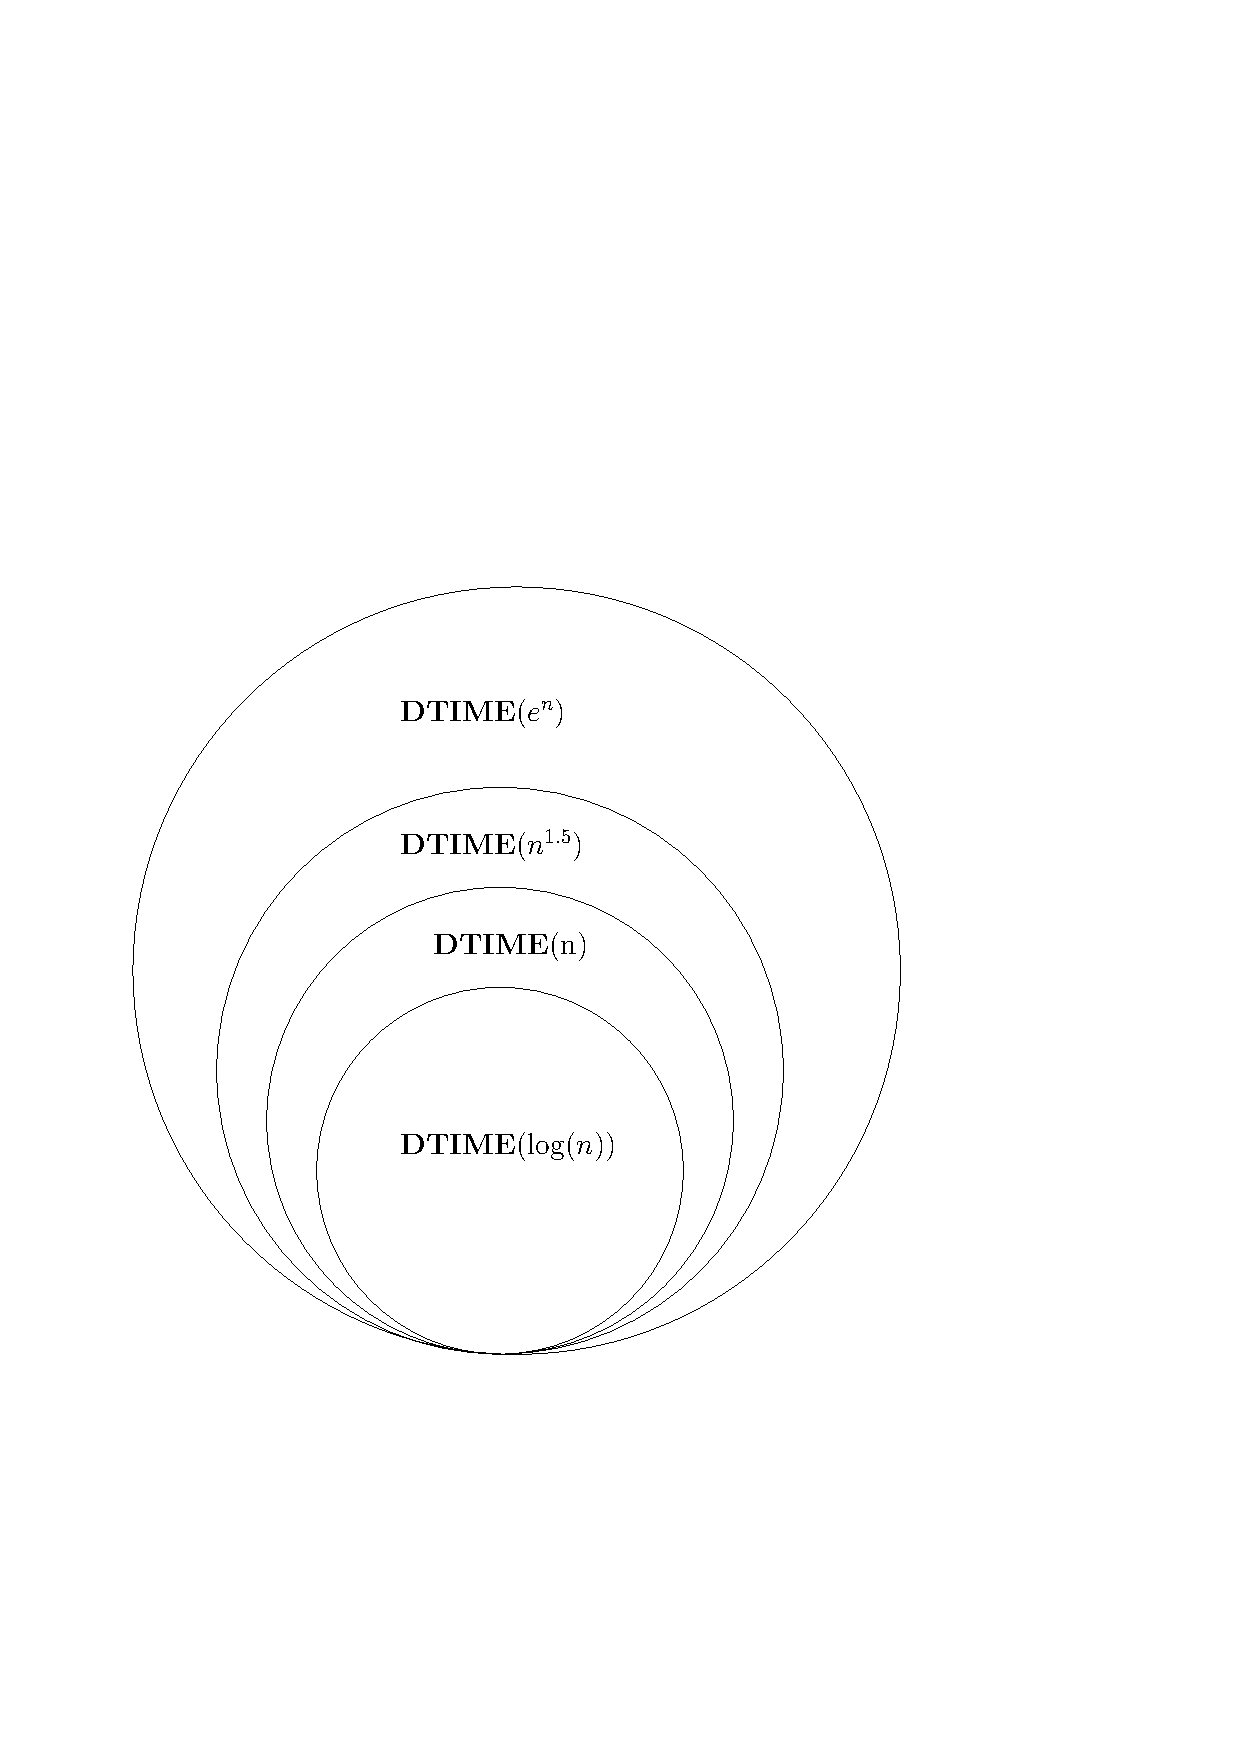
\includegraphics[scale=0.5]{images/timehierarchy.pdf}
\end{frame}

\begin{frame}
	\frametitle{Time Hierarchy}
	\framesubtitle{{Beweis det. Time Hierarchy}}
	Wir zeigen nur $\DTIME(n) \subsetneq \DTIME(n^{1.5})$
	\bigskip
	\pause
	\begin{KITblock}{Definition Turing Maschine D} 
		Bei Eingabe x : Simuliere die TM $M_x$ mit Eingabe x genau für $|x|^{1.4}$ 						Schritte. Danach gebe folgendes aus :
		\begin{equation}
		D(x) = 
		\begin{cases}
			\overline{M_x(x)} & \text{falls die Simulation eine Ausgabe hatte} \\
			0 & \text{sonst}
			
		\end{cases}
		\end{equation}			
	\end{KITblock}
	\bigskip
	\pause	
	
	\begin{KITblock}{Die von D erzeugte Sprache}
		Sei L = $ \lbrace x \vert D(x) = 1  \rbrace$
	\end{KITblock}
\end{frame}

\begin{frame}
	\frametitle{Time Hierarchy}
	\framesubtitle{Beweis det. Time Hierarchy}
	\begin{KITblock}{Behauptung}
		$L \in \DTIME(n^{1.5})$ und $L \notin \DTIME(n)$
	\end{KITblock}
	\pause
	\begin{itemize}[<+->]
		\item Wir nehmen an , dass $L \in \DTIME(n)$
		\item $\Rightarrow \exists$ Turing Maschine M , die L entscheidet und für Eingabe x
		 		höchstens c|x| Schritte benötigt. (c ist konstant)
		\item $\Leftrightarrow \forall x \in {\lbrace 0,1 \rbrace }^{*}$ D(x) = M(x)
	\end{itemize}
\end{frame}

\begin{frame}
	\frametitle{Time Hierarchy}
	\framesubtitle{Beweis det. Time Hierarchy}
	\begin{itemize}[<+->]
		\item Wollen nun M auf D simulieren können
		\item M simuliert auf U läuft in $c|x|\log(|x|)$
		\item Wir wählen dazu $n_0$ so groß, dass $\forall$ $n \geq n_0$ gilt :
			$n^{1.4} > cn\log(n)$		
		\item Nun wählen wir eine Gödelnummer x , so dass $|x| > n_0$ und $M_x$ = M
		\item Nun gilt $D(x) \neq M(x)$ 
		
		\qed 
	\end{itemize}
\end{frame}
